\iffalse
\let\negmedspace\undefined
\let\negthickspace\undefined
\documentclass[journal,12pt,twocolumn]{IEEEtran}
\usepackage{cite}
\usepackage{amsmath,amssymb,amsfonts}
\usepackage{graphicx}
\usepackage{textcomp}
\usepackage{xcolor}
\usepackage{txfonts}
\usepackage{listings}
\usepackage{enumitem}
\usepackage{mathtools}
\usepackage{gensymb}
\usepackage{comment}
\usepackage[breaklinks=true]{hyperref}
\usepackage{tkz-euclide} 
\usepackage{listings}
\usepackage{gvv}                                        
\def\inputGnumericTable{}                                 
\usepackage[latin1]{inputenc}                                
\usepackage{color}                                            
\usepackage{array}                                            
\usepackage{longtable}                                       
\usepackage{calc}                                             
\usepackage{multirow}                                         
\usepackage{hhline}                                           
\usepackage{ifthen}                                           
\usepackage{lscape}
\usepackage[export]{adjustbox}
\usepackage{pgfplots}
\newtheorem{theorem}{Theorem}[section]
\newtheorem{problem}{Problem}
\newtheorem{proposition}{Proposition}[section]
\newtheorem{lemma}{Lemma}[section]
\newtheorem{corollary}[theorem]{Corollary}
\newtheorem{example}{Example}[section]
\newtheorem{definition}[problem]{Definition}
\newcommand{\BEQA}{\begin{eqnarray}}
	\newcommand{\EEQA}{\end{eqnarray}}
\newcommand{\define}{\stackrel{\triangle}{=}}
\newtheorem{rem}{Remark}

\begin{document}
	\parindent 0px
	\bibliographystyle{IEEEtran}
	
	\vspace{3cm}
	
	\title{GATE:EE/63}
	\author{EE23BTECH11208 - Manohar K$^{*}$
	}
	\maketitle
	\newpage
	\bigskip
	
	% \renewcommand{\thefigure}{\theenumi}
	% \renewcommand{\thetable}{\theenumi}
	
	
	
\textbf{Question:} For the closed loop system shown , the transfer function $\frac{E(s)}{R(s)}$ is \\
\begin{figure}[ht]
	\centering
	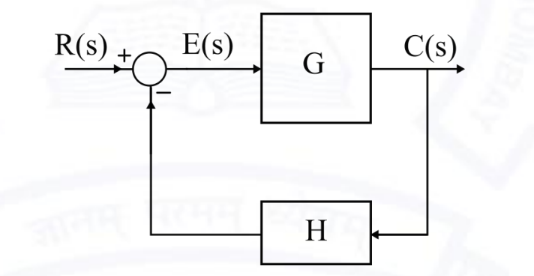
\includegraphics[width=1\linewidth]{2021/EE/11/figs/questiondia.png}
\end{figure}
\begin{enumerate}[label = (\alph*)]
	\item $\frac{G}{1+GH}$
	\item $\frac{GH}{1+GH}$
	\item $\frac{1}{1+GH}$
	\item $\frac{1}{1+G}$
\end{enumerate} \hfill{(GATE EE 2021)}\\



 \noindent \textbf{Solution:}
 \fi
	Given,\\
	
	\begin{table}[h]
		\centering
		
\begin{tabular}{|c|c|}
	\hline
	\textbf{symbol} & \textbf{description} \\
	\hline
	$G$ & Forward path gain\\
	\hline
	$H$ & Feedback path gain\\
	\hline
	$R(s)$ & Input signal \\
	\hline
	$C(s)$ & Output signal \\
	\hline
	$E(s)$ & Error signal \\
	\hline
\end{tabular}
		\caption{Parameters}
		\label{tab:GATE.EE.2021.11}
	\end{table}
	
	\begin{align}
		C(s)&=G \times E(s)\\
		\text{Feedback signal} &= H \times C(s)
	\end{align}
	    
	
	\begin{align}
	      E(s) &= R(s) - H \times C(s)
	\end{align}
	from eq (1),     
	\begin{align}
		E(s) &= R(s) - H \times G \times E(s)
	\end{align}
	\begin{align}
		E(s) +  H \times G \times E(s) &= R(s)
		\end{align}
		\begin{align}
					\therefore \frac{E(s)}{R(s)} &= \frac{1}{1 + GH}
	\end{align} 
	
	
	

